\documentclass{article}
\usepackage[utf8]{inputenc}
\usepackage[T1]{fontenc}
\usepackage{booktabs}
\usepackage{caption}
\usepackage{graphicx}
\usepackage{multirow}
\usepackage{parskip}
\usepackage{hyperref}

\newcommand{\tabitem}{~~\llap{\textbullet}~~}
\def \cmossensoroutputgenerator {\texttt{cmos\_sensor\_output\_generator} }

\title{CMOS Sensor Output Generator}
\author{Sahand Kashani}
\date{\today}

\begin{document}

\maketitle

\section{Core Overview}
The \cmossensoroutputgenerator core is an interface that generates the signals a CMOS sensor would normally output. The core is useful for testing CMOS sensor acquisition systems when the production sensor is not yet available.

The core is configurable at runtime through an Avalon Memory-Mapped (Avalon-MM) interface, and provides a Conduit interface identical to one a CMOS sensor would have.

Additionally, the core comes with a set of C library interfaces that can be used to configure it, as well as to start and stop its operation.

\section{Generated Waveform}
A CMOS sensor outputs 4 signals with which it is possible to sample its data:
\texttt{
    \begin{itemize}
        \itemsep-0.5em
        \item clock
        \item frame\_valid (1-bit)
        \item line\_valid (1-bit)
        \item data (n-bit)
    \end{itemize}
}

Figure~\ref{fig:cmos_sensor_signals_waveform} shows the relationship between the different signals for 2 frames that contain 2 rows and 3 columns each.

The \cmossensoroutputgenerator behaviour can be summarized as follows: The unit outputs sequentially increasing values as pixel data. The first pixel of each frame is assigned the value 0. This value is incremented for each subsequent pixel in the frame.

The maximum possible value is determined by the bit width of the unit's \texttt{data} output port. If the maximum value is smaller than the number of pixels in a frame, the output wraps around and restarts counting from 0.

This guarantees a deterministic output and allows one to verify CMOS sensor acquisition systems for correct behaviour.

\begin{figure}[h]
    \centering
    \makebox[\textwidth][c]{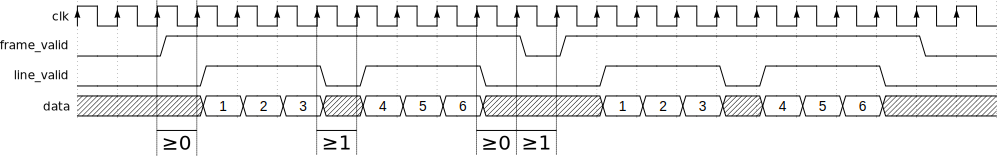
\includegraphics[width=1.3\textwidth]{fig/cmos_sensor_signals_waveform}}%
    \caption{CMOS sensor output signals for two $2\times3$ frames with a pixel depth of 3 bits. Spacing requirements between the various signals are specified in clock cycles. The labels given to the 4 spacing intervals are the same ones used later in Section~\ref{sec:register_map} to configure the core.}
    \label{fig:cmos_sensor_signals_waveform}
\end{figure}

\section{Block Diagram}
Figure~\ref{fig:cmos_sensor_output_generator_external} shows a high-level view of the core.
The \texttt{frame\_valid}, \texttt{line\_valid}, and \texttt{data} signals are generated with the same clock frequency as the core's input clock.

\begin{figure}[h]
    \centering
    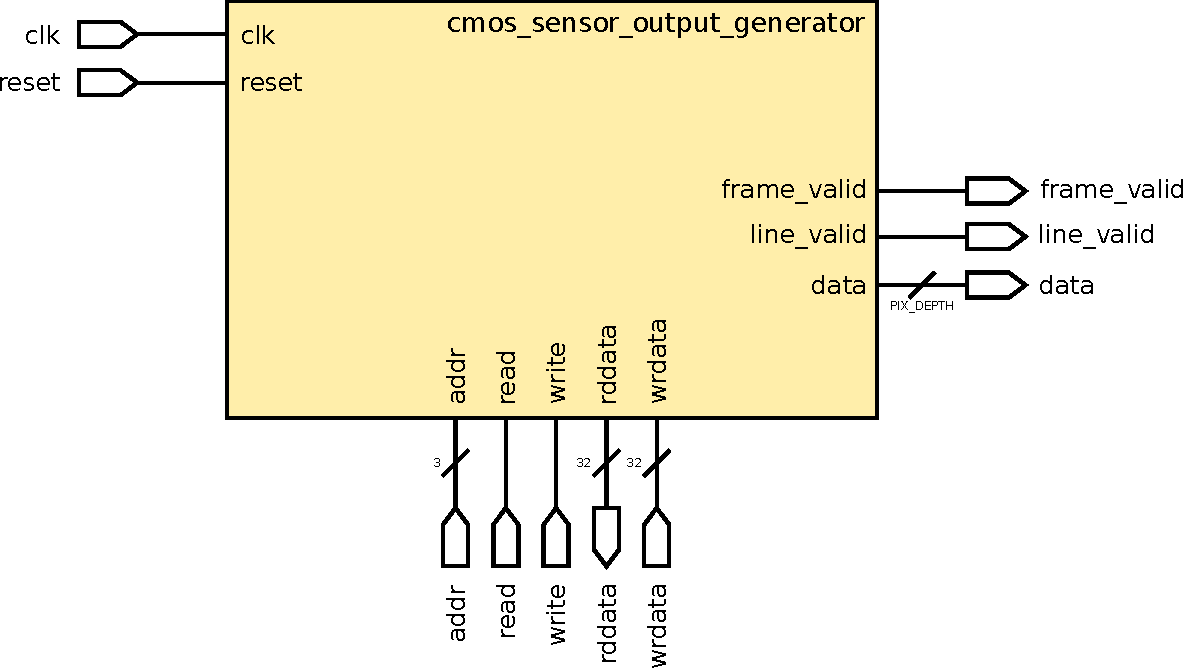
\includegraphics[width=0.9\textwidth]{fig/cmos_sensor_output_generator_external}
    \caption{Block diagram.}
    \label{fig:cmos_sensor_output_generator_external}
\end{figure}

Note that the core does not output the clock it receives as input as a normal CMOS sensor would do, because it is bad practice to route a clock from an FPGA's clock tree through standard logic in order to output it outside the clock tree.

It is the user's responsibility to use the same clock that is driving the core for any other component down the acquisition pipeline that requires the CMOS sensor's generated output clock.

\section{Register Map}
\label{sec:register_map}
The core is configured through multiple \texttt{CONFIG\_} registers, shown in Table~\ref{tab:register_map}. If a configuration register is written with a value smaller than those specified in column \texttt{Minimum}, then the core has undefined behaviour.
\begin{table}[h]
    \centering
    \texttt{
        \begin{tabular}{cclcc}
            \toprule
            Offset & Type & Name                        & Default Value & Minimum \\
            \midrule
            0x00   & RW   & CONFIG\_FRAME\_WIDTH        & 1             & 1       \\
            0x04   & RW   & CONFIG\_FRAME\_HEIGHT       & 1             & 1       \\
            0x08   & RW   & CONFIG\_FRAME\_FRAME\_BLANK & 1             & 1       \\
            0x0C   & RW   & CONFIG\_FRAME\_LINE\_BLANK  & 0             & 0       \\
            0x10   & RW   & CONFIG\_LINE\_LINE\_BLANK   & 1             & 1       \\
            0x14   & RW   & CONFIG\_LINE\_FRAME\_BLANK  & 0             & 0       \\
            0x18   & WO   & COMMAND                     & N/A           & N/A     \\
            0x1C   & RO   & STATUS                      & N/A           & N/A     \\
            \bottomrule
        \end{tabular}
    }
    \caption{Register map. Note that the \texttt{CONFIG\_} registers can only be modified if the core is not running (you must issue a \texttt{STOP} command before modifying any of these registers).}
    \label{tab:register_map}
\end{table}

You can start or stop the controller by writing a command to its \texttt{COMMAND} register, shown in Table~\ref{tab:command_register}. Upon reception of a \texttt{STOP} command, the controller halts immediately and does not wait for the current frame to end.

\begin{table}[h]
    \centering
    \texttt{
        \begin{tabular}{ccl}
            \toprule
            Name  & Value & Description      \\
            \midrule
            STOP  & 0     & Stop generation  \\
            START & 1     & Start generation \\
            \bottomrule
        \end{tabular}
    }
    \caption{\texttt{COMMAND} Register Definitions.}
    \label{tab:command_register}
\end{table}

The \texttt{STATUS} register is described in Table~\ref{tab:status_register}.

\begin{table}[h]
    \centering
    \texttt{
        \begin{tabular}{ccl}
            \toprule
            Name & Value & Description     \\
            \midrule
            BUSY & 0     & Controller busy \\
            IDLE & 1     & Controller idle \\
            \bottomrule
        \end{tabular}
    }
    \caption{\texttt{STATUS} Register Definitions.}
    \label{tab:status_register}
\end{table}

\newpage

\section{Qsys Interface}
Figure~\ref{fig:qsys_gui} shows the Qsys configuration interface for the core.
\begin{figure}[h]
    \centering
    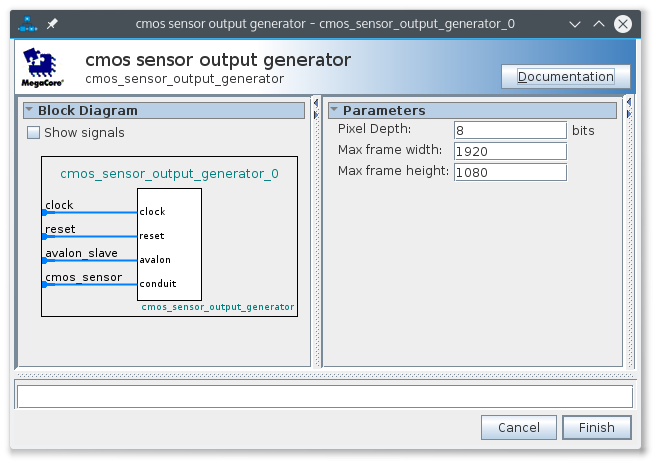
\includegraphics[width=1.0\textwidth]{fig/qsys_gui}
    \caption{Qsys Configuration Interface.}
    \label{fig:qsys_gui}
\end{figure}


Three paramters are needed to instantiate the core:

\begin{itemize}
    \item \texttt{Pixel depth}
    \item \texttt{Max frame width}
    \item \texttt{Max frame height}
\end{itemize}

The \texttt{Max frame width} and \texttt{Max frame height} entries are used to determine the size of the internal registers. This helps keep the unit's footprint small if small resolutions are required.

\end{document}
